\chapter{Referencial Teórico}
\label{cap:referencial}

Esse capítulo aborda os principais conceitos envolvidos no trabalho,  como computação paralela, o modelo MapReduce, sua implementação de código aberto Hadoop e algoritmos de ordenação paralela.

\section{Computação Paralela}

A computação paralela constitui-se de uma coleção de elementos de processamento que se comunicam e cooperam entre si e com isso resolvem um problema de maneira mais rápida \cite{Almasi:1994}. Mesmo com o avanço tecnológico das últimas décadas, as arquiteturas sequenciais de Von Neumann ainda demostram deficiências quando utilizadas por aplicações que necessitam de grande poder computacional. Essa necessidade de maior poder computacional causou o surgimento da computação paralela, com a proposta de aumentar o poder computacional das máquinas.

No estudo de computação paralela, é importante diferenciar os conceitos de paralelismo e concorrência, que podem ser confundidos, pois ambos tratam de programação e execução de tarefas em múltiplos fluxos, implementados com o objetivo de resolver um único problema. Concorrência consiste de diferentes tarefas serem executadas ao mesmo tempo, de forma a produzir um resultado particular mais rapidamente. Isso não implica na existência em múltiplos elementos de processamento; a concorrência pode ocorrer tanto com um único processador quanto com múltiplos processadores. 
Por outro lado, o paralelismo exige a execução de várias tarefas simultaneamente, com a necessidade de vários elementos de processamento. 
Se há apenas um elemento de processamento não há paralelismo, pois apenas uma tarefa será executada a cada instante, mas pode haver concorrência, pois o processador pode ser compartilhado pelas tarefas em execução \cite{Breshears:2009}.

% Desafios da computação paralela e medidas de desempenho
Comparada à computação sequencial, a computação paralela apresenta alto desempenho e soluções mais naturais para problemas intrinsecamente paralelos, mas sua utilização também inclui algumas desvantagens. Há muito mais detalhes e diversidades no desenvolvimento, uma vez que um programa paralelo envolve múltiplos fluxos de execução simultâneos e é preciso coordenar todos os fluxos para completar uma dada computação. Além disso, o desenvolvimento de soluções paralelas apresenta maior dificuldade na programação, necessidade de balanceamento de cargas, sincronismo e intensa sobrecarga de comunicação \cite{Rauber:2010} . 

O desenvolvimento de software paralelo introduz três principais desafios: assegurar confiabilidade de software, minimizar o tempo de desenvolvimento e conquistar bom desempenho na aplicação \cite{Leiserson:2008}.

Manter a confiabilidade do sistema é essencial, pois ao se introduzir paralelismo a aplicação se torna vulnerável às condições de corrida, e dependendo da ordem de execução das tarefas o software pode se comportar de forma diferente. Mesmo se nenhuma alteração for feita no hardware ou nos arquivos de entrada, execuções consecutivas da mesma aplicação podem produzir resultados diferentes. Lidar com situações como essa é particularmente desafiante, pois tais erros são assíncronos e ocorrem eventualmente, o que os torna difíceis de evitar e de encontrar durante testes.

Outro desafio é minimizar o tempo de desenvolvimento, já que muitas vezes o desenvolvimento paralelo é mais complexo que sequencial. Além do maior tempo para escrever o código, a depuração é mais trabalhosa e diversos testes devem ser feitos no sistema, o que pode dispender maior tempo.

O bom desempenho da aplicação é um objetivo central da paralelização, mas pode ser comprometido por comunicação excessiva ou balanceamento irregular de carga. 
O balanceamento de carga busca atingir um aproveitamento ótimo dos recursos do sistema, alocando tarefas de forma a obter o mesmo nível de esforço em todos os processadores. 
A comunicação e sincronização de tarefas são tipicamente as maiores barreiras para se atingir grande desempenho em programas paralelos, e devem ser minimizadas pelo desenvolvedor. Para avaliar o desempenho de algoritmos paralelos, algumas métricas definidas são largamente utilizadas. A lei de Amdahl e a eficiência são os principais indicadores de desempenho de algoritmos paralelos. 

A lei de Amdahl demonstra que o ganho de desempenho que pode ser obtido melhorando uma parte do sistema é limitado pela fração de tempo em que essa parte é utilizada pelo sistema. Pode ser utilizada para calcular o ganho de desempenho de uma máquina, conhecido como \textit{speedup} \cite{Amdahl:1967}.
O \textit{speedup} determina a relação existente entre o tempo gasto para executar um algoritmo de maneira sequencial em um único processador ($T_{sequencial}$) e o tempo gasto para executá-lo em $p$ processadores (T$_{paralelo}$): $ speedup = T_{sequencial}/T_{paralelo}$.
O \textit{speedup} ideal é aquele igual a $p$, que significaria um aumento da capacidade de processamento é diretamente proporcional ao número de processadores. O resultado do \textit{speedup}
pode ser diretamente afetado por fatores como comunicação entre processos, granulosidades inadequadas e partes não paralelizáveis de programas.
 
A eficiência é outro parâmetro utilizados para medir o desempenho quando se utiliza computação paralela. Ela relaciona o \textit{speedup} ao número de processadores, identificando a taxa de utilização do processador. Pode ser calculada por: $E_p = speedup/p$. Em uma paralelização ideal, a eficiência tem valor 1, significando que os processadores têm utilização total.

\subsection{Modelos de programação paralela}

Um modelo de programação descreve um sistema de computação paralela em termos da semântica da linguagem ou do ambiente de programação. Seu objetivo é fornecer um mecanismo com o qual o programador pode especificar programas paralelos. Os tradicionais modelos de programação paralela são: memória compartilhada, passagem de mensagens, paralelismo de dados e de tarefas (\textit{threads}/\textit{multithreads}). 

No ambiente de memória compartilha, múltiplos processadores compartilham o espaço de endereçamento de uma única memória. A comunicação entre os processos é implícita, pois a memória é acessível diretamente por todos os processadores. O paralelismo de dados é o modelo de programação no qual as várias tarefas realizam operações em elementos distintos de dados, simultaneamente, e então trocam dados globalmente.

No ambiente \textit{multithread}, múltiplas \textit{threads} podem ser executadas dentro de um único processo. Cada \textit{thread} possui seu próprio conjunto de registradores e pilha, porém compartilha o mesmo espaço de endereçamento, temporizadores e arquivos, de forma natural e eficiente com as demais \textit{threads} do processo. 

O modelo de memória distribuída consiste em vários processadores, cada um com sua própria memória, interconectados por uma rede de comunicação, como representado na Figura \ref{fig:ArquiteturaDistribuida}.
Nesse modelo as tarefas compartilham dados por meio de comunicação de envio e recebimento de mensagens. Essa passagem de mensagens pode ser realizada por meio de bibliotecas como a MPI (\textit{Message Passing Interface}) e a PVM (\textit{Parallel Virtual Machine}) \cite{Rauber:2010}. 

\begin{figure}[htb]
\centering
%trim left, bottom, right and top
\includegraphics[trim=0cm 1cm 0cm 0cm, width=0.5\textwidth]{figuras/Arquitetura.pdf}
\caption{Modelo de arquitetura distribuída}
\label{fig:ArquiteturaDistribuida}
\end{figure}

\subsection{Computação paralela em \textit{clusters}}
Com o avanço tecnólogico da última década, o volume crescente de dados sendo gerado, coletado e armazenado tornou o processamento dos dados inviável a um único computador. A quantidade de dados atualmente processados cria a necessidade de computação de alto desempenho, cujo foco sejam os dados.  Como resultado, torna-se crucial substituir a computação tradicional por computação distribuída eficiente, e é um caminho natural para o processamento de dados em larga escala o uso de \textit{clusters} ~\cite{Lin:2010}.

\textit{Clusters} são conjuntos de máquinas, ligadas em rede, que comunicam-se através do sistema, trabalhando como se fossem uma única máquina de grande porte. 
Dentre algumas características observadas em um \textit{cluster}, é possível destacar: o baixo custo se comparado a supercomputadores; a proximidade geografica dos nós; altas taxas de transferência nas conexões entre as máquinas e o uso de máquinas em geral homogêneas \cite{Toth:2008}.

Apesar dos computadores em um \textit{cluster} não precisarem processar necessariamente a mesma aplicação, a grande vantagem de tal organização é a habilidade de cada nó processar individualmente uma fração da aplicação, resultando em desempenho que pode ser comparado ao de um supercomputador.
Em geral os computadores de \textit{clusters} são de baixo custo, o que permite que um grande número de máquinas seja interligado, garantindo desempenho e melhor custo-benefício que supercomputadores, o que apresenta outra vantagem. Além disso, novas máquinas podem ser facilmente incorporadas  ao \textit{cluster}, tornando-o uma solução mais flexível, principalmente por ser formado por máquinas de capacidade de processamento similar.

O bom desempenho das aplicações em \textit{clusters} envolve conceitos relacionados à infraestrutura, principalmente comunicação entre os nós e balanceamento de carga.
Para que o processamento do \textit{cluster} possa ser utilizado de maneira eficiente, é importante que os dados a serem processados sejam transferidos suficientemente rápidos para evitar que os processadores fiquem ociosos, através de redes de alta velocidade \cite{Rauber:2010}. 


\subsection{Computação paralela em grandes volumes de dados}
O processamento em \textit{clusters} é uma tarefa cujo desempenho é dependente de diversos fatores, como descrito anteriormente. O processamento de grandes volumes de dados também é uma tarefa desafiadora, que tem sido objeto de vários estudos. O processamento deve ser baseado em alguns princípios para garantir a escalabilidade e o bom desempenho.

A coleta e manutenção dos dados deve ser funções do sistema e não tarefa dos usuários. O sistema deve prover tratamento intrínseco dos dados  e os usuários devem ter facilidade para acessar os dados. Mecanismos de confiabilidade, como replicação e  correção de erros devem ser incorporados como parte do sistema, de modo a garantir integridade e disponibilidade dos dados.

O uso de modelos de programação paralelo de alto nível também deve ser incentivado. O desenvolvedor deve utilizar programação de alto nível que não inclua configurações específicas de uma máquina. O trabalho de distribuir a computação entre as máquinas de forma eficiente deve ficar a cargo do sistema, e não do desenvolvedor.

%Os usuários devem ser capazes de executar programas de forma interativa, com variação dos requisitos de computação e armazenamento. O sistema deve responder rapidamente à consultas e cálculos simples, e não degradar o desempenho geral quando a tarefa for complexa. 
%Para suportar a computação interativa, deve haver oferta de recursos. O custo consequente do aumento dos recursos ofertados pode ser justificado com base no aumento da produtividade dos usuários do sistema.

Além disso, um sistema para computação de grandes volumes de dados deve implementar mecanismos de confiabilidade, no qual os dados originais e intermediários são armazenados de forma redundante. Isso permite que no caso de falhas de componente ou dados seja possível refazer a computação. Além disso, a máquina deve identificar e desativar automaticamente componentes que falharam, de modo a não prejudicar o desempenho do sistema e se manter sempre disponível \cite{Bryant:2011}.

Grandes empresas de serviços de Internet - como Google, Yahoo!, Facebook e Amazon - buscam soluções para processamento de dados em grandes conjuntos de máquinas que atendam as características descritas, pois com um software que provê tais características é possível alcançar alto grau de escalabilidade e custo-desempenho. 

Dentre as principais propostas está o modelo MapReduce e sua implementação Hadoop, que são soluções escaláveis, capazes de processar grandes volumes de dados, com alto nível de abstração para distribuir a aplicação e mecanismos de tolerância a falhas.
A próxima seção apresenta com mais detalhes o modelo e suas características.

\section{MapReduce}
O MapReduce é um modelo de programação paralela criado pela Google para processamento de grandes volumes de dados em \textit{clusters}. Esse modelo propõe simplificar a computação paralela e ser de fácil uso, abstraindo conceitos complexos da paralelização - como tolerância a falhas, distribuição de dados e balanço de carga - e utilizando duas funções principais: Map e Reduce. A complexidade do algoritmo paralelo não é vista pelo desenvolvedor, que pode se ocupar em desenvolver a solução proposta \cite{Dean:2008}.

Esse modelo de programação é inspirado em linguagens funcionais, tendo como base as primitivas Map e Reduce.
Os dados de entrada são específicos para cada aplicação e descritos pelo usuário.
A função Map é aplicada aos dados de entrada e produz uma lista intermediária de pares (chave, valor). Todos os valores intermediários associados a uma mesma chave são agrupados e enviados à função Reduce.
A função Reduce é então
%aplicada a todos os pares intermediários com a mesma chave. A função
combina esses valores para formar um conjunto menor de resultados.
Tipicamente, há apenas zero ou um valores de saída em cada função Reduce. A saída de cada função é agrupada e forma um conjunto de pares no formato (chave, valor).

O pseudocódigo a seguir apresenta um exemplo de uso do MapReduce, cujo objetivo é contar a quantidade de ocorrências de cada palavra em um documento. A função Map recebe como valor uma linha do documento texto, e como chave o número da linha. Para cada palavra encontrada na linha recebida, a função emite a palavra e a contagem de uma ocorrência. A função Reduce, recebe como chave uma palavra, e uma lista dos valores emitidos pela função Map, associados com a palavra questão. As ocorrências da palavra são agrupadas e a função retorna palavra e seu total de ocorrências.

\begin{lstlisting}[label=some-code,caption=some-code]
Function Map (Integer chave, String valor):
	#chave: número da linha no arquivo.
	#valor: texto da linha correspondente.
	listaDePalavras = split (valor)
	for palavra in listaDePalavras:
		emit (palavra, 1)
Function Reduce (String chave, Iterator valores):
	#chave: palavra emitida pela função Map.
	#valores: conjunto de valores emitidos para a chave.
	total = 0
	for v in valores:
		total = total + 1
	emit (palavra, total)
\end{lstlisting}

A Figura \ref{fig:MapReduceexemplo} ilustra o fluxo de execução para este exemplo. A entrada é um arquivo contendo as linhas "hadoop conta", "conta palavras" e "exemplo hadoop".

\begin{figure}[htb]
\centering
%trim left, bottom, right and top
\includegraphics[trim=0cm 9cm 0cm 1cm, width=\textwidth]{figuras/MapReduceExemplo.pdf}
\caption{Fluxo simplificado da contagem de palavras com o MapReduce}
\label{fig:MapReduceexemplo}
\end{figure}

\subsection{Arquitetura do MapReduce}
O MapReduce é constituído de uma arquitetura com dois tipos principais de nós: \textit{Master} e \textit{Worker}. O nó mestre tem como função atender requisições de execução dos usuários, gerenciá-las, criar tarefas e distribuí-las entre os nós trabalhadores, que executam as tarefas com base nas funções Map e Reduce definidas pelo usuário.
%Como é possível perceber, trata-se de uma típica arquitetura mestre-escravo (do inglês master-slave) (DUBREUIL; GAGNÉ; PARIZEAU, 2006).
A arquitetura também inclui um sistema de arquivos distribuídos, onde ficam armazenados os dados de entrada e intermediários.
%Para evitar a transferência excessiva de dados, os \textit{workers} do MapReduce são também nós do sistema de arquivos.


% }

\subsection{Visão geral do fluxo de execução}


As chamadas da função Map são distribuídas automaticamente entre as diversas máquinas através do particionamento dos dados de entrada em \textit{M} conjuntos. Cada conjunto pode ser processado em paralelo por diferentes máquinas. As chamadas da função Reduce são distribuídas pelo particionamento do conjunto intermediário de pares em \textit{R} partes. O número de partições \textit{R} pode ser definido pelo usuário.

A Figura \ref{fig:MapReduceoverview} ilustra uma o fluxo de uma execução do modelo MapReduce \cite{Dean:2008}. A sequência de ações descrita a seguir explica o que ocorre em cada um dos passos. A numeração dos itens a seguir corresponde à numeração da figura.

 \begin{figure}[!htb]
 \centering
%trim left, bottom, right and top
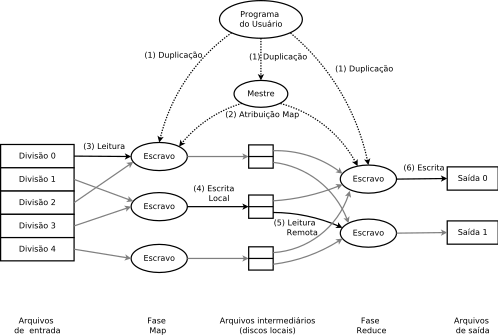
\includegraphics[trim=0cm 2cm 0cm 1cm, width=\textwidth]{figuras/MapReduceOverflow.pdf}
\caption{Visão geral do funcionamento do modelo MapReduce.}
\label{fig:MapReduceoverview}
\end{figure}

\begin{enumerate}
\item A biblioteca MapReduce, no programa do usuário, primeiro divide os arquivos de entrada em M pedaços. Em seguida, iniciam-se muitas cópias do programa para o conjunto de máquinas;

\item Uma das cópias do programa é especial: o mestre (\textit{Master}). Os demais são trabalhadores (\textit{Workers}) cujo trabalho é atribuído pelo mestre. Existem M tarefas Map e R tarefas Reduce a serem atribuídas. O mestre atribui aos trabalhadores ociosos uma tarefa Map ou uma tarefa Reduce;

\item Um trabalhador que recebe uma tarefa Map lê o conteúdo do fragmento de entrada correspondente. Ele analisa pares (chave, valor), a partir dos dados de entrada e encaminha cada par para a função Map definida pelo usuário. Os pares (chave, valor) intermediários, produzidos pela função Map, são colocados no \textit{buffer} de memória;

\item Periodicamente, os pares colocados no \textit{buffer} são gravados no disco local, divididos em regiões R pela função de particionamento. As localizações desses pares bufferizados no disco local são passadas de volta para o mestre, que é responsável pelo encaminhamento desses locais aos trabalhadores Reduce;

\item Quando um trabalhador Reduce é notificado pelo mestre sobre essas localizações, ele usa chamadas de procedimento remoto para ler os dados no \textit{buffer}, a partir dos discos locais dos trabalhadores Map. Quando um trabalhador Reduce tiver lido todos os dados intermediários para sua partição, ela é ordenada pela chave intermediária para que todas as ocorrências da mesma chave sejam agrupadas. Se a quantidade de dados intermediários é muito grande para caber na memória, um tipo de ordenação externa é usado;

\item O trabalhador Reduce itera sobre os dados intermediários ordenados e, para cada chave intermediária única encontrada, passa a chave e o conjunto correspondente de valores intermediários para função Reduce do usuário. A saída da função Reduce é anexada a um arquivo de saída final para essa partição Reduce;

             	        	
\end{enumerate}

Após todas as tarefas Map e Reduce concluídas, o mestre acorda o programa do usuário. Neste ponto, a chamada MapReduce no programa do usuário retorna para o código do usuário.

\section{Hadoop}
Uma das implementações mais conhecidas do MapReduce é o Hadoop, desenvolvido por Doug Cutting em 2005 e mantido pela Apache Software Foundation. O Hadoop é uma implementação código aberto em Java do modelo criado pela Google, que provê o gerenciamento de computação distribuída, de maneira escalável e confiável \cite{Hadoop:2010}.

Facebook, Yahoo! e eBay utilizam o ambiente Hadoop em seus \textit{clusters} para processar diariamente terabytes de dados e logs de eventos para detecção de \textit{spam}, \textit{business intelligence} e diferentes tipos de otimização \cite{Cherkasova:2011}.

O modelo MapReduce foi criado para permitir o processamento em conjuntos de centenas de máquinas de maneira transparente, o que significa que o usuário não deve ser preocupar com mecanismos de tolerância a falhas, que deve ser provido pelo sistema \cite{Dean:2008}. 
Um dos principais benefícios do Hadoop é a implementação desse mecanismo de tolerância a falhas, sejam elas de disco, processos, ou de nós, o que permite que o trabalho do usuário possa ser concluído.

O sistema é capaz de verificar e substituir nós quando ocorre alguma falha. O nó mestre envia mensagens periódicas aos demais nós para verificar seus estados. Se nenhuma resposta é recebida, o mestre identifica que houve uma falha neste nó. 
As tarefas que não foram executadas são reescalonadas para os demais nós. O mecanismo de replicação garante que sempre haja um número determinado de cópias dos dados, e caso um dos nós de armazenamento seja perdido, os demais se encarregam de realizar uma nova replicação \cite{Hadoop:2010}.



\subsection{Sistema de Arquivos do Hadoop}


O \textit{ Hadoop Distributed File System} (HDFS) é um sistema de arquivos distribuído desenvolvido para armazenar grandes conjuntos de dados e ser altamente tolerante a falhas \cite{Hadoop:2010}.
A plataforma Hadoop é compatível com diversos sistemas de arquivos distintos, como Amazon S3 (Native e Block-based), CloudStore, HAR, Local (destinado a unidades de armazenamento conectadas localmente) e sistemas mantidos por servidores FTP e HTTP, mas fornece o HDSF como sistema de arquivos padrão.

A arquitetura do HDFS também é do tipo mestre-escravos.
O nó mestre (\textit{NameNode}) é responsável por manter e controlar todos os metadados do sistema de arquivos e gerenciar a localização dos dados. Também é responsável por outras atividades, como por exemplo, balanceamento de carga, \textit{garbage collection}, e atendimento a requisições dos clientes.
Os nós escravos (\textit{DataNode}) são responsáveis por armazenar e transmitir os dados aos usuários que os requisitarem.

A Figura \ref{fig:hdfs} ilustra a arquitetura do sistema de arquivos distribuídos.
O \textit{NameNode} gerencia e manipula todas as informações dos arquivos, tal como a localização e o acesso. Os \textit{DataNodes} se encarregam da leitura e escrita das informações nos sistemas de arquivos cliente. Os conceitos de nó \textit{Master} e \textit{Worker} do MapReduce, são respectivamente denominados \textit{JobTracker} e \textit{TaskTracker} no Hadoop.
\begin{figure}[htb]
\centering
%trim left, bottom, right and top
\includegraphics[trim=0cm 6cm 0cm 2cm, width=0.6\textwidth]{figuras/HadoopCluster.pdf}
\caption{Visão abstrata do cluster.}
\label{fig:hdfs}
\end{figure}

O HDFS incorpora funcionalidades que têm grande impacto no desempenho geral do sistema.
Uma delas é conhecida como \textit{rack awareness}. Com esse recurso, o sistema de arquivos é capaz de identificar os nós escravos que pertencem a um mesmo \textit{rack}, e distribuir as réplicas de maneira mais inteligente, aumentando o desempenho e a confiabilidade do sistema.
A outra funcionalidade é a distribuição dos dados. O sistema de arquivos busca manter um balanceamento na ocupação das unidades de armazenamento, e o \textit{framework} busca atribuir tarefas a um \textit{worker} que possua, em sua unidade de armazenamento local, os dados que devem ser processados.
Assim, quando executa-se grandes operações MapReduce com um número significativo de nós, a maioria dos dados são lidos localmente e o consumo de banda é mínimo.



\section{Ordenação de dados}


%
%Um grande número de aplicações paralelas possui uma fase de computação intensa, na qual uma lista de elementos deve ser ordenada com base em algum de seus atributos. Um exemplo é o algoritmo de Page Rank \cite{Page:1999} da Google: as páginas de resultado de uma consulta são classificadas de acordo com sua relevância, e então precisam ser ordenadas de maneira eficiente \cite{Kale:2010}.
%No exemplo do Page Rank, o número de páginas a serem ordenadas é enorme, e elas são recolhidas de diversos servidores da Google; é uma questão fundamental escolher algoritmo paralelo com o melhor desempenho dentre as soluções possíveis.
%
%Na criação de algoritmos de ordenação paralela, é ponto fundamental ordenar coletivamente os dados de cada processo individual, de forma a utilizar todas as unidades de processamento e minimizar os custos de redistribuição de chaves entre os processadores.
%\label{cap:ordenacao}
%
%\begin{itemize}
%\item importância da ordenação paralela
%\item formas de ordenação: memória e disco
%\item grandes dados: apenas disco
%\item grandes dados: problematização (tempo, limite de memória)
%\item grandes dados: sort benchmark
%\end{itemize}
%
%
%\begin{itemize}
%\item algoritmos de ordenação paralelos
%\item funcionamento geral
%\item condições / ingredientes / limites
%\item diferentes algoritmos para diferentes aplicações
%\item descrição de algoritmos (e diagramas): sample sort, quick sort
%
%\end{itemize}

A ordenação é o processo de organizar elementos de uma sequência em determinada ordem, e é um dos problemas fundamentais na computação devido à sua importância teórica e prática. De forma geral, a ordenação pode ser dividida em dois grupos: a ordenação interna e externa. 
A ordenação em memória interna é caracterizada pelo armazenamento de todos os registros na memória principal, onde seus acessos são feitos diretamente pelo processador. Essa ordenação é possível apenas quando a quantidade de dados é pequena o suficiente para ser armazenada em memória. 

Quando é preciso ordenar uma base de dados muito grande, que não cabe na memória principal, um outro modelo faz-se necessário, a ordenação externa.
Apesar do problema nos dois casos ser o mesmo - rearranjar os registros de um arquivo em ordem ascendente ou descendente - não é possível usar as mesmas estratégias da ordenação interna, pois o acesso aos dados precisa ser feito em memória secundária, como discos, cujo tempo de acesso é superior ao da memória principal.  %[Ziviani 2007, Knuth 1973].

Na ordenação externa, os itens que não estão na memória principal devem ser buscados em memória secundária e trazidos para a memória principal, para assim serem comparados. Esse processo se repete inúmeras vezes, o que o torna lento, uma vez que os processadores ficam grande parte do tempo ociosos à espera da chegada dos dados à memória principal para serem processados. Por esse motivo, a grande ênfase de um método de ordenação externa deve ser na minimização do número de vezes que cada item é transferido entre a memória interna e a memória externa. Além disso, cada transferência deve ser realizada de forma tão eficiente quanto as características dos equipamentos disponíveis permitam \cite{Ziviani:2007}.



\section{Algoritmos de Ordenação Paralela}

A ordenação paralela é o processo  de ordenação feito em múltiplas unidades de processamento, que trabalham em conjunto para ordenar uma sequência de entrada. O conjunto inicial é dividido em subconjuntos disjuntos, que são associados a uma única unidade de processamento. A sequência final ordenada é obtida a partir da composição dos subconjuntos ordenados. É um ponto fundamental do algoritmo de ordenação paralela que a ordenação feita por cada processo individual seja organizada de tal forma que todas as unidades de processamento estejam trabalhando, enquanto o custo de redistribuição de chaves entre os processadores é minimizado. 

 
Diversas soluções de ordenação podem ser consideradas ao implementar um algoritmo de ordenação em ambiente paralelo. Cada uma delas atende um cenário, tipo de entrada, plataforma ou arquitetura particulares. Dessa forma, ao implementar algoritmos de ordenação paralela, é importante considerar certas condições que interferem no desempenho final do algoritmo, relacionadas tanto ao ambiente de implementação, quanto ao conjunto de dados que deve ser ordenado. As principais questões a serem analisadas são \cite{Kale:2010}:

\begin{itemize}
\item \textbf{Habilidade de explorar distribuições iniciais parcialmente ordenadas:}
Alguns algoritmos podem se beneficiar de cenários nos quais a sequência de entrada dos dados é mesma, ou pouco alterada. Nesse caso, é possível obter melhor desempenho ao realizar menos trabalho e movimentação de dados.
Se a alteração na posição dos elementos na sequência é pequena o suficiente, grande parte dos processadores mantém seus dados iniciais e precisa se comunicar apenas com os processadores vizinhos.

\item \textbf{Movimentação dos dados:}
A movimentação de dados entre processadores deve ser mínima durante a execução do algoritmo. Em um sistema de memória distribuída, a quantidade de dados a ser movimentada é um ponto crítico, pois o custo de troca de dados pode dominar o custo de execução total e limitar a escalabilidade.

\item \textbf{Balanceamento de carga:}
O algoritmo de ordenação paralela deve assegurar o balanceamento de carga ao distribuir os dados entre os processadores. Cada processador deve receber uma parcela equilibrada dos dados para ordenar, uma vez que o tempo de execução da aplicação é tipicamente limitada pela execução do processador mais sobrecarregado.

\item \textbf{Latência de comunicação:}
A latência de comunicação é definida como o tempo médio necessário para enviar uma mensagem de um processador a outro.
Em grandes sistemas distribuídos, reduzir o tempo de latência se torna muito importante.

\item \textbf{Sobreposição de comunicação e computação:}
Em qualquer aplicação paralela, existem tarefas com focos em computação e comunicação. A sobreposição de tais tarefas permite que sejam feitas tarefas de processamento e ao mesmo tempo operações de entrada e saída de dados, evitando que os recursos fiquem ociosos durante o intervalo de tempo necessário para a transmissão da carga de trabalho.

\end{itemize}


Além das condições relacionadas à implementação do algoritmo em ambiente paralelo, existem outras condições necessárias, relacionadas principalmente às propriedades do conjunto de elementos a ser ordenado. Considerando um conjunto de elementos $ \tau = {k_1, k_2, ... , k_n} $ distribuído entre $p$ processadores, é preciso que durante a execução de qualquer algoritmo de ordenação paralela todas as chaves da sequência inicial sejam preservadas, ou seja, que não se perca nenhuma chave durante a distribuição entre os processadores. É necessário ainda que o conjunto de chaves seja particionada em $p$ subconjuntos mutualmente exclusivos, sem nenhuma chave duplicada e que o conjunto de todas as chaves satisfaça as propriedades de um conjunto parcialmente ordenado (Adicionar propriedades do conjunto parc ord).

Após o conjunto estar ordenado, é preciso verificar se todas as chaves da sequência inicial foram preservadas, se todas as chaves de cada processador estão ordenadas em ordem crescente, se a maior chave no processador $p_{i}$ é inferior ou igual ao menor chave no processador $p_{i+1}$ e se a saída resultante é uma sequência de chaves totalmente ordenada.


\subsection{Fluxo geral de execução da ordenação paralela}

Na execução de um algoritmo de ordenação paralela, podem ser identificadas algumas tarefas principais, normalmente realizadas de forma sequencial, que todos os algoritmos precisam executar em algum momento \cite{Kale:2010}. 
A primeira tarefa é a ordenação local, na qual as chaves em cada processador são ordenadas inicialmente, ou ordenadas em grupos.
Existe também uma fase de agrupamento, pois muitas vezes é necessário colocar as chaves em grupos, a fim de enviá-las a outros processadores ou calcular histogramas. Por fim, é preciso realizar a intercalação das chaves ordenadas em subsequências em uma sequência completa.

%visto pela perspectiva da comunicação, pode ser generalizada, uma vez que estão submetidos às mesmas limitações. 
%A fim de fazer uma generalização sobre o fluxo de controle de algoritmos de ordenação, algumas tarefas 

De forma geral, todos os algoritmos de ordenação paralela executam tarefas similares que podem ser definidas, de maneira superficial, como se segue: 
\\1. Realizar processamento local;
\\2. Coletar informações relevantes de distribuição de todos os processadores;
\\3. Em um único processador, inferir uma divisão de chaves a partir das informações coletadas;
\\4. Transmitir aos outros processadores a divisão dos elementos;
\\5. Realizar processamento local;
\\6. Mover os dados de acordo com os elementos de divisão;
\\7. Realizar processamento local;
\\8. Se a divisão de chaves foi incompleta, retornar ao passo 1;


De acordo com essa generalização, é possível identificar pontos que se relacionam diretamente com as condições que limitam o desempenho dos algoritmos de ordenação paralela, e fornecem ideias para a análise de eficiência da comunicação dos algoritmos. 
Primeiro, há duas funções principais de comunicação: descobrir um vetor de divisão global e enviar os dados para os processadores adequados. 
Em segundo lugar, a maioria dos algoritmos têm múltiplos estágios de computação local e pode ser muito vantajoso sobrepor este processamento local e a comunicação. 
%Finalmente, se é possível realizar sobreposição entre o processamento local e a determinação do vetor de divisão, um processador pode ser reservado para o trabalho de divisão, encurtando o caminho crítico. 
O custo da comunicação necessária em um algoritmo (para determinar a divisão e mover os dados) e o custo do processamento local que pode ser sobreposto à essa comunicação é um bom indicativo para comparação da escalabilidade dos algoritmos de ordenação paralela.

%4.1.1 General terminology
%The following terms will be used repeatedly throughout the solution section.
%• n - total number of elements to be sorted.
%• p - number of processing units
%• Π[1,p] - unsorted initial sequences. Processing unit k posseses Πk for k ∈ [1, p].
%• len[1,p] - length of initial sequences. Πk has length k fork∈[1,p].
%• Ξ[1,p] - sorted final sequences. Processing unit k poss- esesΞk fork∈[1,p].
%• flen[1,p] - length of final sequences. Ξk has length flenk fork∈[1,p].
%• threshold - the maximum number of extra keys each
%processor can end up with. More precisely, for all k ∈
%[1, p], f lenk ≤ n + threshold. p

%4.1.2 Splitting of data
%A fundamental problem of parallel sorting is ensuring that each Ξk has a continuous portion of the entire key set. This requirement is necessary to achieve globally sorted order over all processors. The requirement could be rephrased to say that for k ∈ [2,p − 1], Ξk has all existing keys in the range [Sptr[k − 1], Sptr[k]], Ξ1 has all keys smaller than Sptr[1] and, Ξp has all keys larger than Sptr[p − 1]. Sptr is commonly referred to as a splitting vector and has length p−1.
%Most modern parallel sorting algorithms find Sptr explicitly in order to determine what processor each key belongs on. The difficulty lies in that Sptr directly dictates the load balance of the final sequence sizes. As previously mentioned,
%
%f lenk should be smaller than n + threshold for all k ∈ [1, p]. p
%It is therefore necessary to find a splitting vector, Sptr, such that for each of p key ranges generated by elements Sptr, the number of existing keys in the range is smaller than
%n +threshold. p
%At a high level, we can gain the insight that a splitting vector needs to properly relate the distribution of keys within the key range with the corresponding key values.
%There are three commonly used methods for determining the splitting vector, Sptr:
%1. Pre-emptive: Use application-level knowledge to es- tablish Sptr directly. Or, simply assume Sptr to be uniform.
%2. Sample [7] : draw a sample from the global key set and select Sptr from the sample.
%3. Histogram [8]: make a naive guess at Sptr, then iter- atively adjust it by computing how many keys belong to each range.
%Many parallel sorting algorithms use modified versions of these techniques but most use at least one at a high level. Notably, some algorithms do not determine Sptr all at once but rather in multiple iterations or levels of recursion.



\subsection{Sample Sort}

O algoritmo \textit{Sample Sort}, ou Ordenação por Amostragem, é um método de ordenação baseado na divisão do arquivo de entrada em subconjuntos, de forma que as chaves de um subconjunto $i$ sejam menores que as chaves do subconjunto $i+1$. Após a divisão, cada subconjunto é enviado a um processador, que ordena os dados localmente. Ao final, todos os subconjuntos são concatenados e formam um arquivo globalmente ordenado.

Nesse algoritmo, o ponto chave é dividir as partições de maneira balanceada, para que cada processador receba aproximadamente a mesma carga de dados. Para isso, é preciso estimar o número de elementos que devem ser destinados a uma certa partição, que é feita através da amostragem das chaves do arquivo original. Essa estratégia baseia-se na análise de um subconjunto de dados, denominado amostra, ao invés de todo o conjunto, para estimar a distribuição de chaves e, assim, construir partições balanceadas.

Existem três tipos de estratégias de amostragem: \textit{SplitSampler}, \textit{IntervalSampler} e \textit{RandomSampler}. O \textit{SplitSampler} seleciona os $n$ primeiros registros do arquivo para formar a amostra. O \textit{IntervalSampler} cria a amostra com a seleção de chaves em intervalos regulares no arquivo. No \textit{RandomSampler}, a amostra é constituída por chaves selecionadas aleatoriamente no conjunto. A melhor estratégia de amostragem depende diretamente dos dados de entrada. O \textit{SplitSampler} não é recomendado para arquivos quase ordenados, pois as chaves selecionadas serão as iniciais, que não são representativas do conjunto como um todo. Nesse caso, a melhor escolha é o \textit{IntervalSampler} pelo fato de selecionar chaves que representam melhor a distribuição do conjunto. O \textit{RandomSampler} é considerado um bom amostrador de propósito geral [White 2009], e foi utilizado na implementação do algoritmo feito por Pinhão (2011) e utilizado neste trabalho.

Para criar a amostra, o \textit{RandomSampler} necessita de alguns parâmetros, como a probabilidade de escolha de uma chave, o número máximo de amostras a serem selecionadas para realizar a amostragem e o número máximo de partições que podem ser utilizadas.
O número máximo de partições é determinado pelo número de núcleos disponíveis por processador e pela quantidade de máquinas, de acordo com a equação: $particoes$ = $nucleos$ x $maquinas$.
Após a definição das amostras, são conhecidos os intervalos compreendidos por cada partição. As informações das partições são armazenadas em um arquivo e transmitidas para as demais máquinas por meio de cache distribuído.


\subsubsection{Algoritmo em MapReduce}

%A Figura 4.6 apresenta um esquema da estrutura de funcionamento do algoritmo, quando implementado em MapReduce no ambiente Hadoop. O algoritmo pode ser di- vidido em duas fases: Map e Reduce.
%
%Na fase Map, os arquivos de entrada são lidos, ocorre a formação do vetor inicial e dos pares (chave, valor) dos valores lidos (passos 1.1 e 1.2). Depois disso, os dados são divididos em partições cujo número é determinado pelo número de máquinas e seus núcleos de processamento (passo 1.3). No exemplo apresentado, são utilizados dois núcleos de pro- cessamento (cores). Portanto, existem duas partições e, dessa forma, deve ser escolhido apenas um limite para as partições. Esse limite é definido por meio da seleção do ele- mento que melhor representa a distribuição de chaves na amostra formada pela estratégia RandomSampler. Para esse exemplo o limite escolhido foi o número 13, o que implica que em uma partição estarão valores menores e iguais a 13 e, na outra, valores maiores que 13. Por meio de cache distribuído, as informações das partições são transmitidas para as máquinas participantes e os dados particionados. Cada partição é então atribuída a uma tarefa Reduce (processador) diferente.
%
%Na fase Reduce, os dados são ordenados localmente (passo 2.1), ou seja, em cada processador os dados são ordenados na memória interna. Para essa ordenação, avalia-se a profundidade da árvore de recursão e, se ela for baixa, utiliza-se o algoritmo QuickSort. Caso contrário, o HeapSort é utilizado [White 2009]. Após isso, os dados retornam para a máquina master, onde são concatenados, formando o vetor ordenado.O balanceamento das partições, ou seja, a formação de partições aproximadamente iguais no tamanho é muito importante para o algoritmo de Ordenação por Amostragem, pois evita que os tempos de ordenação sejam dominados por um único processador. Em outras palavras, o equilíbrio das partições reduz a possibilidade de que um processador esteja ocioso, enquanto outro processador está sobrecarregado, situação que comprometeria o desempenho do algoritmo [White 2009].

\subsection{Quicksort}

 \subsection{Ordenação no ambiente Hadoop}


A ordenação de dados é uma das cargas de trabalho mais consideradas pelos \textit{benchmarks} em geral, que buscam, a partir de uma entrada desordenada, obter uma saída ordenada de acordo com as chaves de cada par (chave, valor) contido na entrada.
% O \textit{framework} Hadoop disponibiliza diversos programas que podem ser facilmente executados, dentre os quais se destacam o \textit{Sort} e o \textit{TeraSort}.
O \textit{Sort} é um dos mais conhecido dos \textit{benchmarks} de ordenação de dados, definido por Jim Gray em 1998 \cite{Gray:1998}. 
Consiste em um conjunto de seis \textit{benchmarks}, cada um com as suas regras, que medem os tempos para ordenar diferentes números de registros e se diferem princialmente nas métricas de avaliação. 
As principais categorias dos \textit{benchmarks Sort} são a \textit{MinuteSort} e a \textit{GraySort}. A categoria \textit{MinuteSort} deve ordenar a maior quantidade dos dados em um minuto e a \textit{GraySort} deve ordenar mais que 100 terabytes em pelo menos uma hora \cite{White:2009}. Ainda existem as categorias PennySort, JouleSort, e os descontinuados  Datamation Sort e TeraByte Sort. 
Em cada categoria de ordenação, existem duas classificações, de acordo com o tipo de registro a ser ordenado: Daytona e Indy. O participantes da categoria Daytona são códigos de ordenação de propósito geral, e os participantes da Indy devem ordenar apenas registros de 100 bytes, sendo os primeiros 10 bytes de um registro a chave e o restante o valor do elemento a ser ordenado \cite{SortBenchmark}.


No \textit{benchmark Sort} as entradas e saídas devem ser sequências de arquivos onde as chaves e os valores são gravados em byte. 
No Hadoop, o \textit{Sort} é uma aplicação MapReduce, composta de três etapas: gerar dados aleatórios, realizar a ordenação, e validar os resultados.
A geração de dados aleatórios é feita com o programa \textit{RandomWriter}. Ele executa 10 tarefas MapReduce por nó, e cada função Map gera aproximadamente 1GB de dados, totalizando 10GB de dados binários aleatórios, com a chave e os valores de vários tamanhos. É possível alterar o número de dados e as configurações para os tamanhos das chaves e valores, alterando algumas configurações do \textit{RandomWriter}.
O segundo passo é realiza uma ordenação parcial dos dados de entrada, e escrever o resultado em um diretório de saída. 
O passo final é validar os resultados obtidos pela ordenação dos dados realizada pelo \textit{Sort}, através do programa \textit{SortValidator}, que realiza uma série de verificações nos dados ordenados e nos não ordenados para confirmar se a ordenação foi realizada corretamente. Ele relata o estado da validação para o console no final de seu funcionamento, através de uma mensagem de sucesso. 
%:
%\begin{verbatim} %SUCCESS! Validated the MapReduce framework's 'sort' successfully. \end{verbatim}
Esse programa é considerado muito útil para verificar o desempenho do sistema como um todo, uma vez que todo o conjunto de dados é transferido through the shuffle.

%
%
%O Sort é um dos mais conhecidos 
%Os benchmarks relacionados ao Sort possuem uma aplicação MapReduce, que realiza uma ordenação parcial dos dados de entrada, e são constituídos de três passos:
%1. Geração de dados: gera dados aleatórios a serem ordenados;
%2. Ordenação dos dados: ordena os dados gerados pelo passo 1;
%3. Validação de dados: vno passo 2.
%
%

%Hadoop comes with a MapReduce program that does a partial sort of its input. It is very useful for benchmarking the whole MapReduce system, as the full input dataset is transferred through the shuffle. The three steps are: generate some random data, perform the sort, then validate the results.
%First we generate some random data using RandomWriter. It runs a MapReduce job with 10 maps per node, and each map generates (approximately) 10 GB of random binary data, with key and values of various sizes. You can change these values if you like by setting the properties test.randomwriter.maps_per_host and test.random write.bytes_per_map. There are also settings for the size ranges of the keys and values; see RandomWriter for details.

%This command runs the SortValidator program, which performs a series of checks on the unsorted and sorted data to check whether the sort is accurate. It reports the out- come to the console at the end of its run:
%SUCCESS! Validated the MapReduce framework's 'sort' successfully.



// TERASORT


O TeraSort é outra aplicação de destaque para ordenação de dados com Hadoop, criada por Owen O' Malley [O'Malley e Murthy 2009], com o intuito de participar da competição de ordenação chamada GraySort [Gray 1998]. Em 2009, o TeraSort foi o campeão dessa competição em duas categorias, ao ordenar 500 GB em 59 segundos (MinuteSort) utilizando um cluster com 1.406 nodos e 100 TB em 173 minutos (GraySort) em um cluster com 3.452 nodos. A escalabilidade da solução foi provada pela ordenação de 1 PB em 975 minutos (equivalente a 16,25 horas) em 3.658 nodos.

%Outra implementação de destaque para ordenação de dados com Hadoop é a chamada TeraSort, criada por Owen O’ Malley (O’MALLEY; MURTHY, 2009), com o intuito de participar da competição de ordenação chamada GraySort (GRAY et al., 1998). Em 2009, o TeraSort foi o campeão da edição em duas categorias, ao ordenar 500 GB em 1 minuto (MinuteSort) e 100 TB em 173 minutos (GraySort). Para provar a escalabilidade da solução, ainda demonstrou-se os resultados da ordenação de 1 PB em 975 minutos (equivalente a 16,25 horas).
%O TeraSort consiste de três algoritmos, que são responsáveis pela geração dos dados, ordenação e validação. 

\textbf{Teragen} é o programa para geração dados para a ordenação.
O número de registros gerados é um parâmetro definido pelo usuário, assim como número de tarefas Map a serem realizadas. O programa divide o número desejado de registros pelo número de tarefas Map, e atribui intervalos das chaves a cada tarefa para a geração de um arquivo. Cada tarefa Map corresponde a um arquivo de saída,  e os dados gerados são divididos em diversos arquivos. Assim, se existem 2 tarefas Map, serão gerados 2 arquivos, cada um contendo metade das chaves desejadas. 
Os registros gerados têm um formato específico, formado por uma chave, um id e um valor. As  chaves são caracteres aleatórios do conjunto ' ' .. '~'. O id é um valor inteiro que representa a linha, e o valor consiste de 70 caracteres de 'A' a 'Z'. 

\textbf{TeraSort} é uma espécie MapReduce padrão, exceto por um particionador personalizado que usa uma lista ordenada de N-1 chaves amostrados que definem a faixa de chave para cada redução. Em particular, todas as chaves tal que amostra [i-1] <= amostra <chave [i] são enviados para reduzir i. Isto garante que a saída de reduzir i são todos menos do que a saída de reduzir i +1. Para acelerar o particionamento, o particionador constrói uma trie de dois níveis que rapidamente índices para a lista de teclas de amostra com base nos dois primeiros bytes da chave. TeraSort gera as chaves de amostra, por amostragem, a entrada antes do trabalho é apresentado e escrever a lista de chaves em HDFS. Eu escrevi uma entrada e formato de saída, que são utilizados por todos os 3 aplicações, que ler e gravar os arquivos de texto no formato certo. A saída do reduce tem replicação ajustado para 1, em vez do padrão 3, porque a competição não requer os dados de saída para ser replicado em vários nós.
% Na competição, o TeraSort utiliza 1.800 funções Map e Reduce, e outras configurações para que tamanho pilha seja suficiente que os dados transientes nunca foi derramado para outro disco no final do mapa. O amostrador utilizado 100.000 chaves para determinar os limites reduzir, embora, como pode ser visto na Fig.-ure 14-21, a distribuição entre reduz foi quase perfeito e beneficiariam mais amostras. Você pode ver a distribuição de tarefas em execução sobre o trabalho executado na Fig.-ure 14-22.
%

\textbf{TeraValidate} garante que a saída está totalmente ordenada. A aplicação cria uma função Map para cada arquivo no diretório de saida, e cada Map se certifica que cada chave é igual ou menor à anterior. O Map também gera registros com a primeira e última chaves de cada arquivo, e Reduce garante que a primeira chave de arquivo i é maior do que a última chave do arquivo i-1. Todos os problemas são relatados como saída do Reduce, com as chaves que estão fora de ordem.

%TeraGen generates output data that is byte-for-byte equivalent to the C version including the newlines and specific keys. It divides the desired number of rows by the desired number of tasks and assigns ranges of rows to each map. The map jumps the random number generator to the correct value for the first row and generates the following rows. For the final run, I configured TeraGen to use 1,800 tasks to generate a total of 10 billion rows in HDFS, with a block size of 512 MB.
%TeraSort is a standard MapReduce sort, except for a custom partitioner that uses a sorted list of N−1 sampled keys that define the key range for each reduce. In particular, all keys such that sample[i−1] <= key < sample[i] are sent to reduce i. This guarantees that the output of reduce i are all less than the output of reduce i+1. To speed up the partitioning, the partitioner builds a two-level trie that quickly indexes into the list of sample keys based on the first two bytes of the key. TeraSort generates the sample keys by sampling the input before the job is submitted and writing the list of keys into HDFS. I wrote an input and output format, which are used by all 3 applications, that read and write the text files in the right format. The output of the reduce has replication set to 1, instead of the default 3, because the contest does not require the output data be replicated on to multiple nodes. I configured the job with 1,800 maps and 1,800 reduces and io.sort.mb, io.sort.factor, fs.inmemory.size.mb, and task heap size sufficient that transient data was never spilled to disk other at the end of the map. The sampler used 100,000 keys to determine the reduce boundaries, although as can be seen in Fig- ure 14-21, the distribution between reduces was hardly perfect and would benefit from more samples. You can see the distribution of running tasks over the job run in Fig- ure 14-22.
%
%TeraValidate ensures that the output is globally sorted. It creates one map per file in the output directory, and each map ensures that each key is less than or equal to the previous one. The map also generates records with the first and last keys of the file, and the reduce ensures that the first key of file i is greater than the last key of file i−1. Any problems are reported as output of the reduce with the keys that are out of order.